%%%%%%%%%%%%%%%%%%%%%%%%%%%%%%%%%%%%%%%%%
% Beamer Presentation
% LaTeX Template
% Version 1.0 (10/11/12)
%
% This template has been downloaded from:
% http://www.LaTeXTemplates.com
%
% License:
% CC BY-NC-SA 3.0 (http://creativecommons.org/licenses/by-nc-sa/3.0/)
%
%%%%%%%%%%%%%%%%%%%%%%%%%%%%%%%%%%%%%%%%%

%----------------------------------------------------------------------------------------
%	PACKAGES AND THEMES
%----------------------------------------------------------------------------------------

\documentclass[usenames,dvipsnames,table]{beamer}

\mode<presentation> {

\usetheme{Madrid}
%\setbeamertemplate{footline} % To remove the footer line in all slides uncomment this line
%\setbeamertemplate{footline}[page number] % To replace the footer line in all slides with a simple slide count uncomment this line
%\setbeamertemplate{navigation symbols}{} % To remove the navigation symbols from the bottom of all slides uncomment this line
}

\usepackage{graphicx} % Allows including images
\usepackage{booktabs} % Allows the use of \toprule, \midrule and \bottomrule in tables
\usepackage{listings}
\usepackage{enumitem}

%----------------------------------------------------------------------------------------
%	TITLE PAGE
%----------------------------------------------------------------------------------------

\title[ABDA Ex. 2]{Applied Bayesian Data Analysis --- Exercise 3 B}

\author{Kim Albertsson} % Your name
\institute[LTU and CERN]
{
CERN and Luleå University of Technology \\
\medskip
\textit{kim.albertsson@ltu.se}
}
\date{\today}

\newcommand{\cgy}{\cellcolor{gray!25}}
\newcommand{\cgr}{\cellcolor{green!25}}
\newcommand{\cye}{\cellcolor{orange!25}}
\newcommand{\ccb}{\cellcolor{Cerulean!25}}

\begin{document}

\begin{frame}
\titlepage % Print the title page as the first slide
\end{frame}

%----------------------------------------------------------------------------------------
%	PRESENTATION SLIDES
%----------------------------------------------------------------------------------------
\section{Question B.2}
\begin{frame}
\begin{center}
{\huge{Question B.2}}
\\\vspace{2em}
Plot the outcome probabilities given $\theta \in {0.50, 0.25}$ using a bar or a stem plot.
\end{center}
\end{frame}


\begin{frame}[fragile]
Equation for Bernoulli distribution (pdf):
\begin{align*}
p(x|\theta) = \theta^{x} (1-\theta)^{1-x},\ x \in \{0, 1\}
\end{align*}

Code for Bernoulli distribution (pdf):
\begin{lstlisting}[language=Python]
class Bernoulli(object):
    @staticmethod
    def pdf(x, theta=0.5):
        return theta**x * (1-theta)**(1-x)
    @staticmethod
    def likelihood(xs, theta=0.5):
        return np.prod([Bernoulli.pdf(x, theta)
                        for x in xs])
\end{lstlisting}
\end{frame}

\begin{frame}[fragile]
Code for generating plot:
\begin{lstlisting}[language=Python]
plt.figure()
x = [0, 1]
plt.bar(x, Bernoulli.pdf(x, theta=0.25),
        label='$\theta=0.25$', hatch='\\',
        facecolor='none', edgecolor='tab:orange',
        linewidth=2)
plt.bar(x, Bernoulli.pdf(x, theta=0.50),
        label='$\theta=0.25$', hatch='/',
        facecolor='none', edgecolor='tab:orange',
        linewidth=2)
plt.xticks([0, 1], ['$\\theta=0$', '$\\theta=1$'])
plt.ylabel('$p(x|\\theta)$')
plt.legend()
plt.grid()
plt.tight_layout()
\end{lstlisting}
\end{frame}

\begin{frame}
Probability mass for two cases of the Bernoulli distribution:
\begin{figure}
\centering
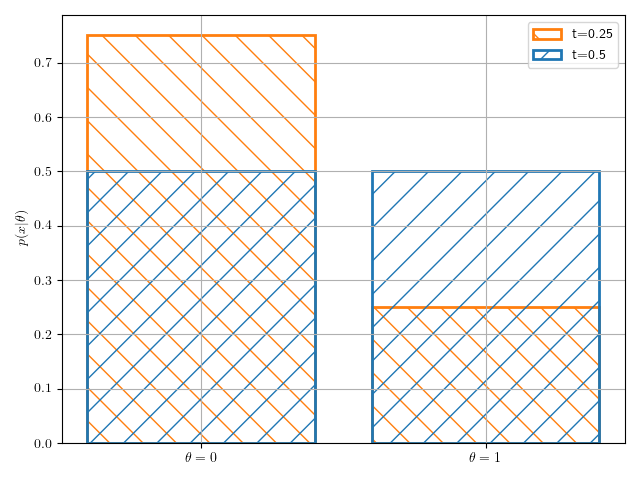
\includegraphics[height=0.8\textheight]{img/ex3B2.png}
\end{figure}
\end{frame}










\section{Question B.3}
\begin{frame}
\begin{center}
{\huge{Question B.3}}
\\\vspace{2em}
Plot the likelihood of a given parameter value $\theta$ given a particular outcome.
\end{center}
\end{frame}

\begin{frame}[fragile]
Code for generating plot:
\begin{lstlisting}[language=Python]
plt.figure()
theta = np.linspace(0, 1, 100)
plt.plot(theta, Bernoulli.pdf(1, theta),
         label='$p(x=1|\\theta)$')
plt.plot(theta, Bernoulli.pdf(0, theta),
         label='$p(x=0|\\theta)$')
plt.xlabel('$\\theta$')
plt.ylabel('$p(\\theta|x)$')
plt.legend()
plt.grid()
plt.tight_layout()
\end{lstlisting}
\end{frame}

\begin{frame}
Likelihoods for two cases of the Bernoulli distribution:
\begin{figure}
\centering
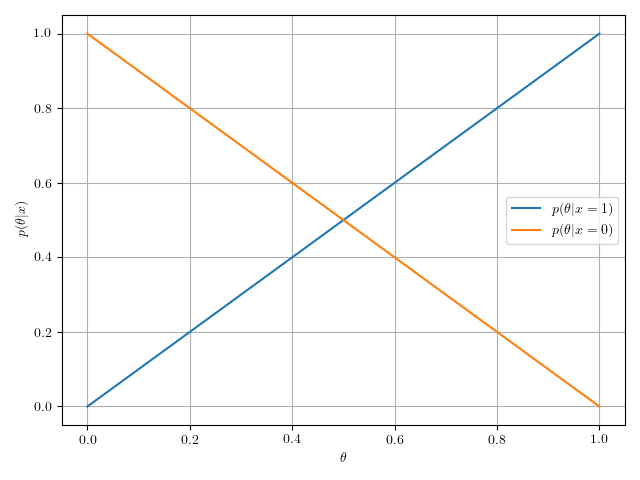
\includegraphics[height=0.8\textheight]{img/ex3B3.png}
\end{figure}
\end{frame}









\section{Question B.4.a}
\begin{frame}
\begin{center}
{\huge{Question B.4.a}}
\\\vspace{2em}
Evaluate the likelihood function for $\theta=0.5$ for $n \in {10, 1000, 100000}$, where $n$ is the number of coin flips in the experiment. What happens for large values of $n$?
\end{center}
\end{frame}

\begin{frame}[fragile]
\textbf{Reminder:} Code for Bernoulli distribution
\begin{lstlisting}[language=Python]
class Bernoulli(object):
    @staticmethod
    def pdf(x, theta=0.5):
        return theta**x * (1-theta)**(1-x)
    @staticmethod
    def likelihood(xs, theta=0.5):
        return np.prod([Bernoulli.pdf(x, theta)
                        for x in xs])
\end{lstlisting}
\end{frame}

\begin{frame}[fragile]
\textbf{Note:} Given $\theta=0.5$, each sequence is equally likely. No need for sampling.
\begin{lstlisting}[language=Python]
>>> Bernoulli.likelihood([0]*10)
0.0009765625
>>> Bernoulli.likelihood([0]*1000)
9.332636185032189e-302
>>> Bernoulli.likelihood([0]*100000)
0.0
\end{lstlisting}

As $n$ tends to infinity, the likelihood tends to zero ($\frac{1}{2}^{-n}$).
\end{frame}




\section{Question B.4.b}
\begin{frame}
\begin{center}
{\huge{Question B.4.b}}
\\\vspace{2em}
Can you evaluate the \emph{log-likelihood} for larger $n$ without problems of under- or overflow?
\end{center}
\end{frame}

\begin{frame}
\textbf{Q:} Why log-likelihood?
\begin{itemize}
\item Computational efficiency, use summation instead of multiplication.
\item \emph{Monotonic} transformation, global minima/maxima coincide.
\end{itemize}

\textbf{Q:} Which log? --- Does it matter? Use binary log for measure in ``bits''?
\end{frame}

\begin{frame}
Equation for Bernoulli distribution (log-pdf):
\begin{align*}
p(x|\theta) &= \theta^{x} (1-\theta)^{1-x},\ x \in \{0, 1\}\\
\log p(x|\theta) &= \log(\theta^{x} (1-\theta)^{1-x})\\
\log p(x|\theta) &= \log\theta^{x}+\log(1-\theta)^{1-x}\\
\log p(x|\theta) &= x\log\theta+(1-x)\log(1-\theta)
\end{align*}
\end{frame}

\begin{frame}[fragile]
Code for Bernoulli distribution (log-pdf)
\begin{lstlisting}[language=Python]
class Bernoulli(object):
    @staticmethod
    def logpdf(x, theta=0.5):
        return (x*np.log(theta) +
                (1-x)*np.log(1-theta))
    @staticmethod
    def loglikelihood(seq, theta=0.5):
        return np.sum([Bernoulli.logpdf(x, theta)
                       for x in seq])
\end{lstlisting}
\end{frame}

\begin{frame}[fragile]
\textbf{Note:} Exact values depend on the base of the logarithm. Your mileage might vary.
\begin{lstlisting}[language=Python]
>>> Bernoulli.loglikelihood([0]*10)
-6.931471805599453
>>> Bernoulli.loglikelihood([0]*1000)
-693.147180559945
>>> Bernoulli.loglikelihood([0]*100000)
-69314.71805599453
\end{lstlisting}

As $n$ tends to infinity, the log-likelihood tends to negative infitnity ($log(\frac{1}{2})n$).
\end{frame}










\section{Question B.4.d-e}
\begin{frame}
\begin{center}
{\huge{Question B.4.d-e}}
\\\vspace{2em}
Plot the likelihood functionwith respect to $\theta$ given $x_0 = [1]; x_0 = [1, 1]; x_2 = [1, 1, 0, 1];$.
\\\vspace{1em}
Explain the behaviour you see in terms of the likelihood of $\theta$ for the particular data sequences.
\end{center}
\end{frame}

\begin{frame}[fragile]
Code for plot:
\begin{lstlisting}[language=Python]
x = np.linspace(0.001, 0.999, 100)
plt.figure()
plt.plot(x, np.exp([Bernoulli.loglikelihood([1], X)
                    for X in x]),
         label='$p(x=[1]|\\theta)$')
plt.plot(x, np.exp([Bernoulli.loglikelihood([1,1], X)
                    for X in x]),
         label='$p(x=[1,1]|\\theta)$')
plt.plot(x, np.exp([Bernoulli.loglikelihood([1,1,0,1],
                                             X)
                 for X in x]),
         label='$p(x=[1,1,0,1]|\\theta)$')
plt.xlabel('$\\theta$')
plt.ylabel('$p(\\theta|x)$')
plt.legend()
plt.grid()
plt.tight_layout()
\end{lstlisting}
\end{frame}

\begin{frame}
\begin{figure}
\centering
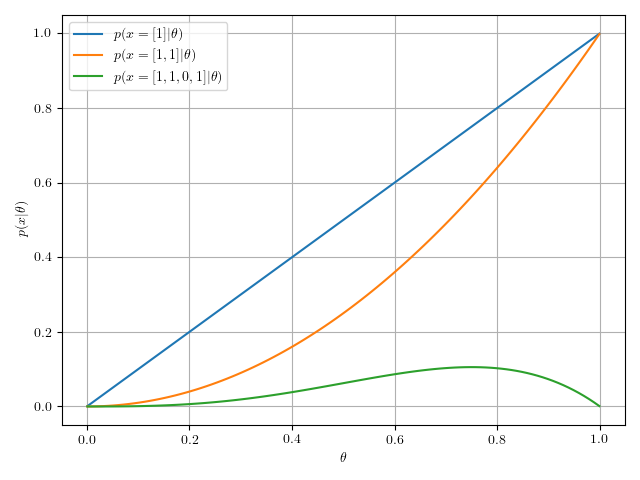
\includegraphics[height=0.7\textheight]{img/ex3B4d.png}
\end{figure}

For $x_2=[1,1,0,1]$: Note that sequence contain both 1's and 0's. Thus the probability for $\theta=0$ and $\theta=1$ are 0. Since more 1's than 0's, maximum skewed towards $\theta=1$.

\end{frame}





\section{Question B.5.a.ii.1-2}
\begin{frame}
\begin{center}
{\huge{Question B.5.a.ii.1-2}}
\\\vspace{2em}
Plot, instead of the likelihoods, the posterior distribution assuming a $p(\theta)=\beta(1,1)$ prior.
\\\vspace{1em}
Compare the mathematical expressions in Eq.~6.1 and Eq.~6.2 with that of Eq.~6.8. Explain differences in plots using this.
\end{center}
\end{frame}

\begin{frame}
Solid lines are posteriors, dashed are likelihoods. Notice the difference in shape.
\begin{figure}
\centering
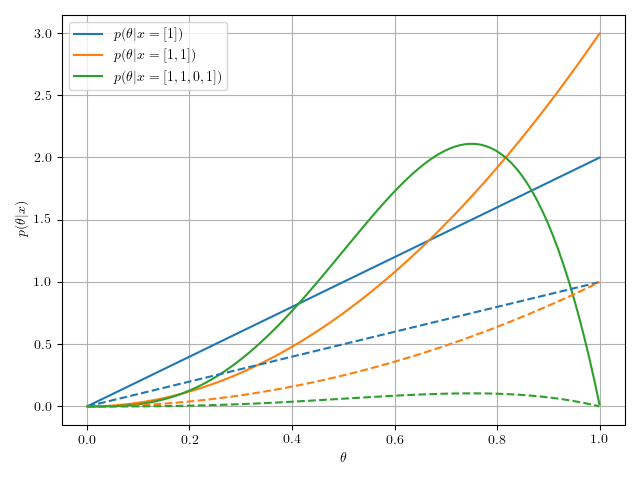
\includegraphics[height=0.8\textheight]{img/ex3B5aii1.png}
\end{figure}
\end{frame}

\begin{frame}
Comparing equations for likelihood (6.2) and posterior (6.8) we see that the difference is a normalisation constant. Note: $N$ is total number of coin flips. $z$ is number of heads.
\begin{align*}
p(\theta) &= \frac{\theta^{1-1}(1-\theta)^{1-1}}{B(1, 1)}\tag{6.3}\\
p(x|\theta) &= \theta^z(1-\theta)^{N-z}\tag{6.2}\\
p(\theta|x) &= \frac{\theta^{z}(1-\theta)^{N-z}}{B(z+1, N-z+1)}\tag{6.8}
\end{align*}
\end{frame}




\section{Question B.5.a.iii}
\begin{frame}
\begin{center}
{\huge{Question B.5.a.iii}}
\\\vspace{2em}
Reproduce Figure~6.4 from the book.
\end{center}
\end{frame}

\begin{frame}[fragile]
Code for plot (1/4):
\begin{lstlisting}[language=Python]
x = np.linspace(0.001, 0.999, 100)
h = 17 # N heads
t = 3  # N tails
y = [1]*h + [0]*t # Data sample

fig, axs = plt.subplots(nrows=3, ncols=3,
                        sharex=True)

axs[0,0].set_title('High belief in prior\n'
                   '$p(\\theta)=\\beta(100,100)$')
axs[0,1].set_title('Balanced\n'
                   '$p(\\theta)=\\beta(18.25,6.75)$')
axs[0,2].set_title('Low belief in prior\n'
                   '$p(\\theta)=\\beta(1,1)$')
\end{lstlisting}
\end{frame}

\begin{frame}[fragile]
Code for plot (2/4):
\begin{lstlisting}[language=Python]
axs[0, 0].fill_between(x,
    np.exp([Beta.logpdf(X, a=100, b=100)
            for X in x]))
axs[0, 0].set_ylabel('$p(\\theta)$')
axs[1, 0].fill_between(x,
    np.exp([Bernoulli.loglikelihood(y, X)
            for X in x]))
axs[1, 0].set_ylabel('$p(x|\\theta)$')
axs[2, 0].fill_between(x,
    np.exp([Beta.logpdf(X, a=117, b=103)
            for X in x]))
axs[2, 0].set_ylabel('$p(\\theta|x)$')
\end{lstlisting}
\end{frame}

\begin{frame}[fragile]
Code for plot (3/4):
\begin{lstlisting}[language=Python]
axs[0, 1].fill_between(x,
    np.exp([Beta.logpdf(X, a=18.25, b=6.75)
            for X in x]))
axs[1, 1].fill_between(x,
    np.exp([Bernoulli.loglikelihood(y, X)
            for X in x]))
axs[2, 1].fill_between(x,
    np.exp([Beta.logpdf(X, a=35.25, b=9.75)
            for X in x]))
\end{lstlisting}
\end{frame}

\begin{frame}[fragile]
Code for plot (4/4):
\begin{lstlisting}[language=Python]
axs[0, 2].fill_between(x,
    np.exp([Beta.logpdf(X, a=1, b=1)
            for X in x]))
axs[1, 2].fill_between(x,
    np.exp([Bernoulli.loglikelihood(y, X)
            for X in x]))
axs[2, 2].fill_between(x,
    np.exp([Beta.logpdf(X, a=1+h, b=1+t)
            for X in x]))
axs[2, 2].set_xlabel('$\\theta$')

# Plus some code for formatting
\end{lstlisting}
\end{frame}

\begin{frame}
\begin{figure}
\centering
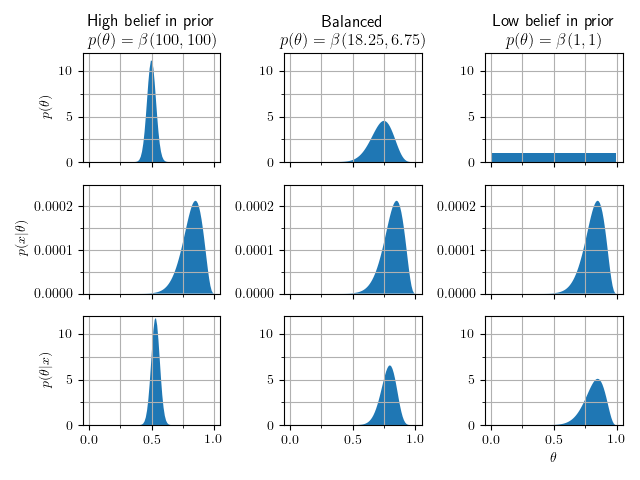
\includegraphics[height=0.8\textheight]{img/ex3B5aiii.png}
\end{figure}
\end{frame}


\section{Appendix}
\begin{frame}
\begin{center}
{\huge{For complete code}}
\\\vspace{2em}
See \url{https://github.com/ashlaban/ltu-abda-2019/tree/master/ex3}
\end{center}
\end{frame}


\end{document} 